\documentclass[
	letterpaper, % Paper size, specify a4paper (A4) or letterpaper (US letter)
	10pt, % Default font size, specify 10pt, 11pt or 12pt
]{CSUniSchoolLabReport}

%----------------------------------------------------------------------------------------
%	REPORT INFORMATION
%----------------------------------------------------------------------------------------

\title{Thevnin Equivalents and Source Transformations \\ Circuits \& Signals \\ EECE2150} % Report title

\author{Michael \textsc{Brodskiy}}

\date{February 13, 2023} % Date of the report

%----------------------------------------------------------------------------------------


\begin{document}

\maketitle % Insert the title, author and date using the information specified above

\begin{center}
	\begin{tabular}{l r}
		Date Performed: & February 6, 2023 \\ % Date the experiment was performed
        Partner: & Juan \textsc{Zapata} \\ % Partner names
		Instructor: & Professor \textsc{Sun} % Instructor/supervisor
	\end{tabular}
\end{center}

\setcounter{section}{-1}

\section{Introduction}

Th purpose of this laboratory experimentation is to apply the concept of the Thevnin equivalent in real world scenarios. Additionally, this lab demonstrates the idea of source transformation.

\section{Part I}

\subsection{Q1} The input resistance of the oscilloscope, measured using the ohmmeter, was approximately $1[\si{\mega\ohm}]$.

\subsection{Q2} The oscilloscope reads $2.5[\si{\volt}]$ across itself — equal to half of the input. This makes sense, because the oscilloscope resistance is roughly equal to the resistance of the resistor in parallel, as shown in figure \ref{fig:1}.

\begin{figure}[H]
  \centering
  \tikzset{every picture/.style={line width=0.75pt}} %set default line width to 0.75pt        

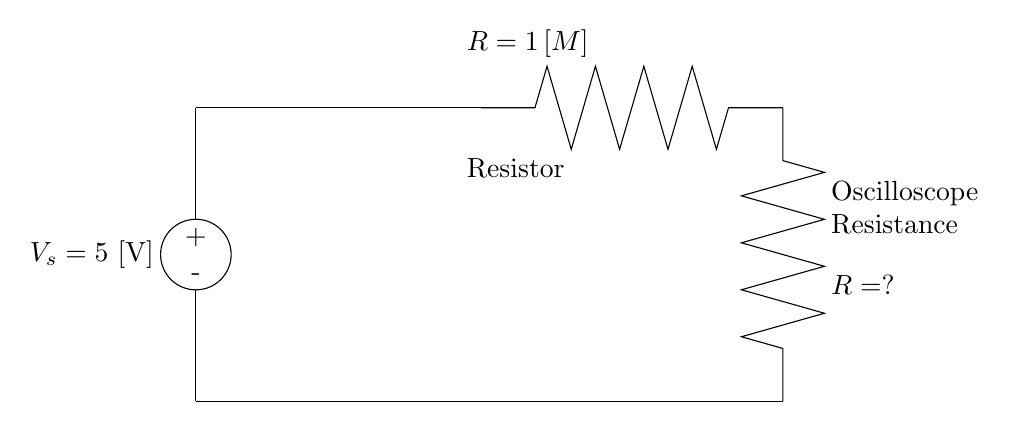
\begin{tikzpicture}[x=0.75pt,y=0.75pt,yscale=-1,xscale=1]
%uncomment if require: \path (0,642); %set diagram left start at 0, and has height of 642

%Shape: Circle [id:dp1293335169248646] 
\draw   (100,140) .. controls (100,130.61) and (107.61,123) .. (117,123) .. controls (126.39,123) and (134,130.61) .. (134,140) .. controls (134,149.39) and (126.39,157) .. (117,157) .. controls (107.61,157) and (100,149.39) .. (100,140) -- cycle ;
%Straight Lines [id:da8573659817175756] 
\draw    (117,69.29) -- (117,123) ;
%Straight Lines [id:da09626430681968268] 
\draw    (117,157) -- (117,210.71) ;
%Straight Lines [id:da19138905725146715] 
\draw    (258.42,69.29) -- (117,69.29) ;
%Straight Lines [id:da9383173165485992] 
\draw    (258.42,210.71) -- (117,210.71) ;
%Straight Lines [id:da51555500958681] 
\draw    (399.84,210.71) -- (258.42,210.71) ;
%Shape: Resistor [id:dp8459054998005646] 
\draw   (254.13,69.29) -- (280.36,69.29) -- (286.19,49.29) -- (297.85,89.29) -- (309.5,49.29) -- (321.16,89.29) -- (332.82,49.29) -- (344.47,89.29) -- (356.13,49.29) -- (367.79,89.29) -- (373.61,69.29) -- (399.84,69.29) ;
%Shape: Resistor [id:dp3577155889138255] 
\draw   (399.84,69.29) -- (399.84,94.75) -- (419.84,100.4) -- (379.84,111.72) -- (419.84,123.03) -- (379.84,134.34) -- (419.84,145.66) -- (379.84,156.97) -- (419.84,168.28) -- (379.84,179.6) -- (399.84,185.25) -- (399.84,210.71) ;

% Text Node
\draw (117,126) node [anchor=north] [inner sep=0.75pt]   [align=left] {\begin{minipage}[lt]{8.68pt}\setlength\topsep{0pt}
\begin{center}
+
\end{center}

\end{minipage}};
% Text Node
\draw (117,154) node [anchor=south] [inner sep=0.75pt]   [align=left] {\begin{minipage}[lt]{8.67pt}\setlength\topsep{0pt}
\begin{center}
\mbox{-}
\end{center}

\end{minipage}};
% Text Node
\draw (98,140) node [anchor=east] [inner sep=0.75pt]   [align=left] {$\displaystyle V_{s} =5$ [V]};
% Text Node
\draw (295.85,92.29) node [anchor=north east] [inner sep=0.75pt]   [align=left] {Resistor};
% Text Node
\draw (307.5,46.29) node [anchor=south east] [inner sep=0.75pt]   [align=left] {$\displaystyle R=1\left[\text{M} \si{\ohm}\right]$};
% Text Node
\draw (421.84,103.4) node [anchor=north west][inner sep=0.75pt]   [align=left] {Oscilloscope\\Resistance};
% Text Node
\draw (421.84,148.66) node [anchor=north west][inner sep=0.75pt]   [align=left] {$\displaystyle R=?$};


\end{tikzpicture}

  \caption{Oscilloscope Equivalent Circuit}
  \label{fig:1}
\end{figure}

\section{Part II} 

\subsection{Q3} The measurements taken (and $R_{TH}$ calculation) are as follows:

\vspace{10pt}

\begin{itemize}

  \item Open Circuit Voltage: $1[\si{\volt}]$

  \item Output Voltage: $\pm.725[\si{\volt}]$

  \item $i_L$: $\dfrac{.725}{100}=7.25[\si{\milli\ampere}]$

  \item $V_L=.275[\si{\volt}]$

  \item $R_{TH}$: $\frac{.275}{7.25}\cdot100=37.93[\si{\ohm}]$

\end{itemize}

\subsection{Q4} The measurements with a $50[\si{\ohm}]$ resistor are:

\begin{itemize}

  \item Output Voltage: $\pm.525[\si{\volt}]$

  \item $i_L$: $\dfrac{.525}{50}=10.5[\si{\milli\ampere}]$

  \item $V_L$: $.475[\si{\volt}]$

\end{itemize}

It makes sense that there is a lower output voltage, as the $50[\si{\ohm}]$ resistor would receive more current and voltage, as compared to the $100[\si{\ohm}]$ resistor.

\section{Part III}

\subsection{Q5} To find the percent, one would calculate the ratio of the found resistance to the sum of the found resistance and oscilloscope resistance, times 100, as follows:

$$\frac{37.93}{37.93+10^6}\cdot100=.0038\%$$

\subsection{Q6} Using the above formula, this would mean that:

$$\dfrac{R_{TH}}{R_{osc}+R_{TH}}\cdot 100 \leq 1$$
$$R_{TH}\leq.01(R_{osc}+R_{TH})$$
$$R_{TH}\leq .0101R_{osc}$$

The oscilloscope needs a resistance of at least 99 times that of the Thevnin resistance.

\section{Source Transformation}

\subsection{Q7} The voltage across $R_2$ is $5[\si{\volt}]$. This matches our voltage divider technique

\subsection{Q8} The graph and table of $R_2$ values are shown below

 \begin{center}
        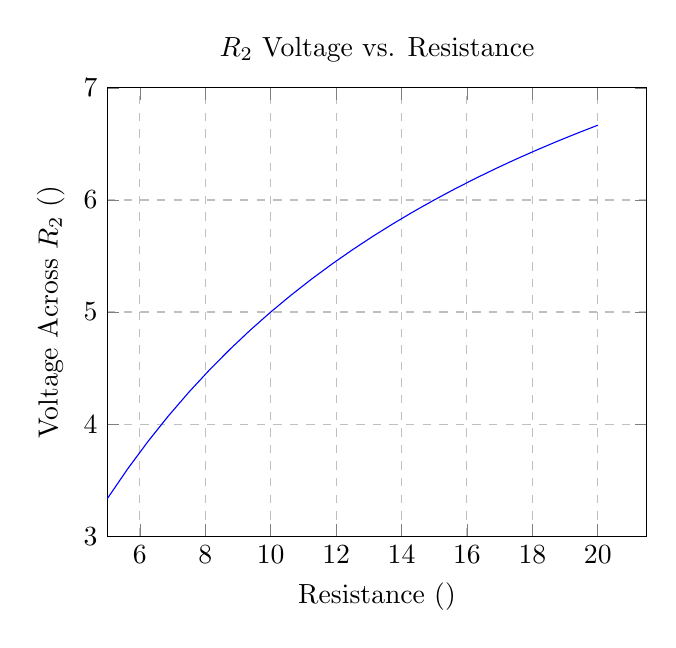
\begin{tikzpicture}
          \begin{axis}[xmin=5, title={$R_2$ Voltage vs. Resistance}, xlabel={Resistance ($\si{\ohm}$)}, ylabel={Voltage Across $R_2$ ($\si{\volt}$)}, ymajorgrids=true, xmajorgrids=true, grid style=dashed]
            \addplot [domain=5:20,blue] {10 * x / (10 + x)};
        \end{axis}
        \end{tikzpicture}
    \end{center}

    \begin{center}
      \begin{tabular}[h!]{| c | c |}
        \hline
        $R_2$ ($\si{\ohm}$) & $R_2$ Voltage ($\si{\volt}$)\\
        \hline
        5 & 3.33\\
        \hline
        6 & 3.75\\
        \hline
        7 & 4.12\\
        \hline
        8 & 4.49\\
        \hline
        9 & 4.74\\
        \hline
        10 & 5\\
        \hline
        11 & 5.24\\
        \hline
        12 & 5.45\\
        \hline
        13 & 5.65\\
        \hline
        14 & 5.83\\
        \hline
        15 & 6\\
        \hline
        16 & 6.15\\
        \hline
        17 & 6.3\\
        \hline
        18 & 6.43\\
        \hline
        19 & 6.55\\
        \hline
        20 & 6.67\\
        \hline
      \end{tabular}
    \end{center}

    \subsection{Q9} Despite the source transformation, the voltage across $R_2$ is the same as in the previous question

    \subsection{Q10} The values are the same as above, and are shown below:

 \begin{center}
        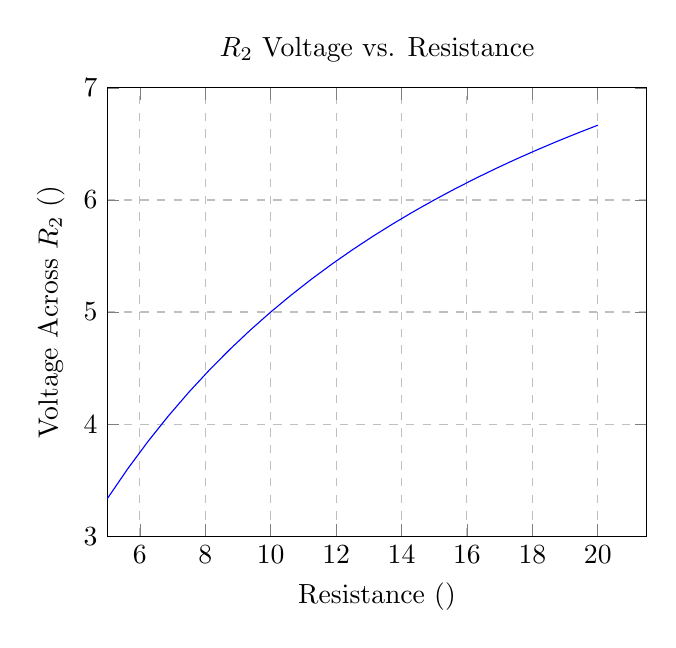
\begin{tikzpicture}
          \begin{axis}[xmin=5, title={$R_2$ Voltage vs. Resistance}, xlabel={Resistance ($\si{\ohm}$)}, ylabel={Voltage Across $R_2$ ($\si{\volt}$)}, ymajorgrids=true, xmajorgrids=true, grid style=dashed]
            \addplot [domain=5:20,blue] {10 * x / (10 + x)};
        \end{axis}
        \end{tikzpicture}
    \end{center}

    \begin{center}
      \begin{tabular}[h!]{| c | c |}
        \hline
        $R_2$ ($\si{\ohm}$) & $R_2$ Voltage ($\si{\volt}$)\\
        \hline
        5 & 3.33\\
        \hline
        6 & 3.75\\
        \hline
        7 & 4.12\\
        \hline
        8 & 4.49\\
        \hline
        9 & 4.74\\
        \hline
        10 & 5\\
        \hline
        11 & 5.24\\
        \hline
        12 & 5.45\\
        \hline
        13 & 5.65\\
        \hline
        14 & 5.83\\
        \hline
        15 & 6\\
        \hline
        16 & 6.15\\
        \hline
        17 & 6.3\\
        \hline
        18 & 6.43\\
        \hline
        19 & 6.55\\
        \hline
        20 & 6.67\\
        \hline
      \end{tabular}
    \end{center}

    \subsection{Q11} The two graphs are identical due to the source transformation performed

    \subsection{Q12} The power dissipated by $R_2$ is equal to:

    $$5[\si{\volt}](.5[\si{\ampere}])=2.5[\si{\watt}]$$

    \subsection{Q13} The graph for power dissipated by $R_2$ is as follows:

 \begin{center}
        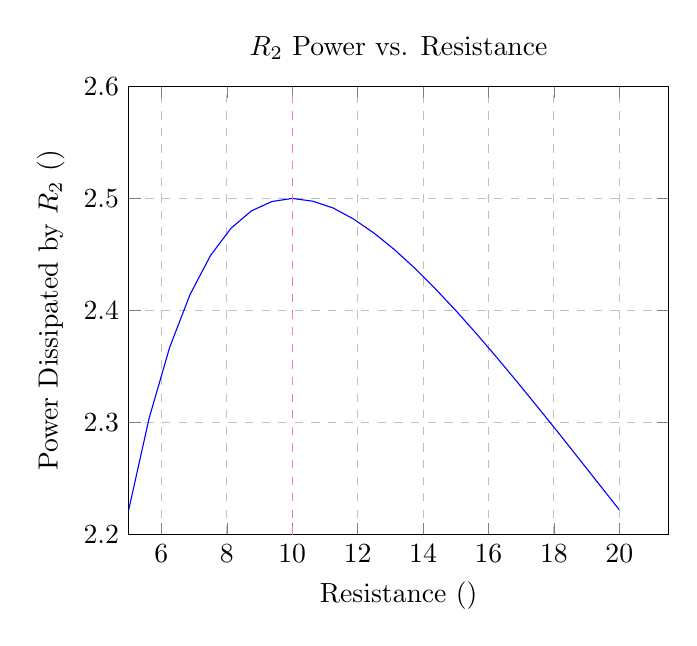
\begin{tikzpicture}
          \begin{axis}[xmin=5, ymin=2.2, ymax=2.6, title={$R_2$ Power vs. Resistance}, xlabel={Resistance ($\si{\ohm}$)}, ylabel={Power Dissipated by $R_2$ ($\si{\watt}$)}, ymajorgrids=true, xmajorgrids=true, grid style=dashed]
            \addplot [domain=5:20,blue] {x * (10 / (10 + x))^2};
            \addplot [dashed,red!50] coordinates {(10,2.2) (10,2.6)};
        \end{axis}
        \end{tikzpicture}
    \end{center}

    \begin{center}
      \begin{tabular}[h!]{| c | c |}
        \hline
        $R_2$ ($\si{\ohm}$) & $R_2$ Power ($\si{\watt}$)\\
        \hline
        5 & 2.22\\
        \hline
        6 & 2.34\\
        \hline
        7 & 2.42\\
        \hline
        8 & 2.47\\
        \hline
        9 & 2.49\\
        \hline
        10 & 2.5\\
        \hline
        11 & 2.49\\
        \hline
        12 & 2.48\\
        \hline
        13 & 2.46\\
        \hline
        14 & 2.43\\
        \hline
        15 & 2.4\\
        \hline
        16 & 2.37\\
        \hline
        17 & 2.33\\
        \hline
        18 & 2.3\\
        \hline
        19 & 2.26\\
        \hline
        20 & 2.22\\
        \hline
      \end{tabular}
    \end{center}

    \subsection{Q14} The graph rises up until roughly $R_2=10[\si{\ohm}]$ and then falls. This means that $R_2=10[\si{\ohm}]$ is a local maxima.

    \subsection{Q15} A graph with $V=5,7,10,$ and $15[\si{\volt}]$ looks as follows:

    \begin{center}
        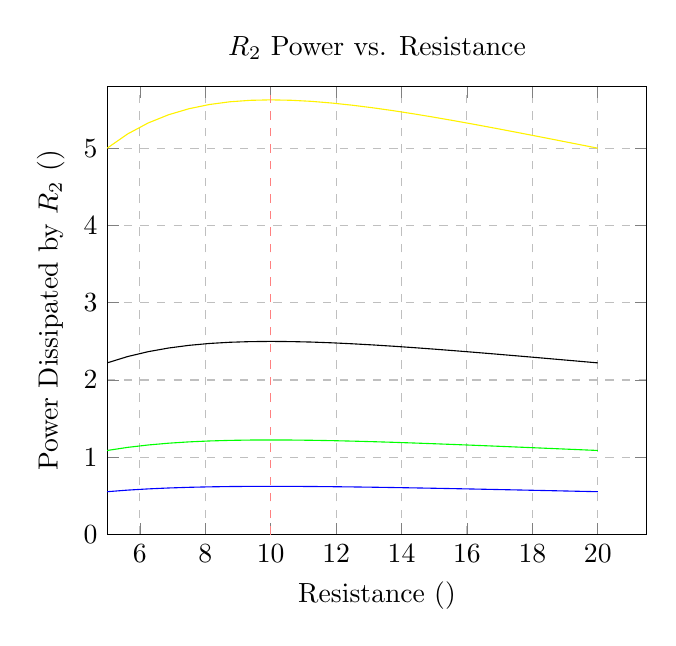
\begin{tikzpicture}
          \begin{axis}[xmin=5, ymin=0, ymax=5.8, title={$R_2$ Power vs. Resistance}, xlabel={Resistance ($\si{\ohm}$)}, ylabel={Power Dissipated by $R_2$ ($\si{\watt}$)}, ymajorgrids=true, xmajorgrids=true, grid style=dashed]
            \addplot [domain=5:20,blue] {x * (5 / (10 + x))^2};
            \addplot [domain=5:20,green] {x * (7 / (10 + x))^2};
            \addplot [domain=5:20,black] {x * (10 / (10 + x))^2};
            \addplot [domain=5:20,yellow] {x * (15 / (10 + x))^2};
            \addplot [dashed,red!50] coordinates {(10,0) (10,7)};
        \end{axis}
        \end{tikzpicture}
    \end{center}

    The plots all have maximums at $10[\si{\ohm}]$. This is most likely because, at this value, the voltage splits most uniformly between the two resistors.

\section{Conclusion}

Overall, this laboratory experiment allowed us to determine the Thevnin equivalent circuit of the classroom oscilloscope. In doing so, the concept of Thevnin equivalents was demonstrated to us through real world means. On top of this, the correctness of source transformation was confirmed.

\end{document}
